\documentclass[9pt,t,aspectratio=169]{beamer}
\usetheme{metropolis}
\usepackage{style/slide}
\usepackage{listings}
\usepackage{amsmath}
\usepackage[default]{lato}
\usepackage[T1]{fontenc}

\title{Hermite Polynomial Features for Private Data Generation}

\subtitle{ᡤᡠᠯᡠ-ᡧᠠᠩᡤᡳᠶᠠᠨ-ᡤᡡᠰᠠ}
\date{}
\author{Seongho Joo}
\institute{SNU MILAB}

\begin{document}
\begin{frame}{Warm-up}
\begin{define}[Gegenbauer polynomial]
The Gegenbauer polynomial of degree $\ell \geq 0$ in dimension $d \geq 2$ is given by 
\begin{equation*}
    P_d^{\ell} (t) := \sum_{j=0}^{\floor{\ell /2}} c_j \cdot t^{\ell -2j} \cdot (1-t^2)^j 
\end{equation*}
where $c_0 = 1$ and $c_{j+1} = -\frac{(\ell -2j) (\ell -2j -1)}{2 (j+1)(\red{d}-1+2j)}c_j$ for $j=0,1, \dots, \floor{\ell/2}-1$. 
\end{define}
Chebyshev polynomials $(d=2)$, Legendre polynomials $(d=3)$, monomials ($d=\infty)$. 
\begin{enumerate}
    \item (Orthogonality)  
    \begin{equation*}
        \int_{-1}^{-1} P_d^{\ell} (t) P_d^{\ell^{\prime}}(t) (1-t^2)^{\frac{d-3}{2}} \dd{t} = \frac{\abs{\bS^{d-1}}\mathbf{1}_{\set{\ell = \ell^{\prime}}}}{\alpha_{\ell, d} \cdot \abs{\bS^{d-2}}}
    \end{equation*}
    \item (Reproducing property) For any $x,y, \in \bS^{d-1}$, 
    \begin{equation*}
        P_d^{\ell} (\inner{x}{y}) = \alpha_{\ell, d} \cdot \E_{w \sim \cU(\bS^{d-1})} \left[ P_d^{\ell} (\inner{x}{w}) P_d^{\ell}( \inner{y}{w}) \right]. 
    \end{equation*}
\end{enumerate}
\end{frame}
\begin{frame}{}
    \begin{define}[Generalized zonal kernels] For an integers $s \geq 1$ and a sequence of vector-valued functions $h_{\ell}: \real \to \real^s$ for $\ell=0,l1, \dots$, we define the generalized zonal kernel (GZK) of order $s$ as 
\begin{equation*}
    k(x,y) := \sum_{\ell =0}^{\infty} \inner{h_{\ell} ( \norm{x})}{h_{\ell} (\norm{y})} P_d^{\ell} \left( \frac{\inner{x}{y}}{\norm{x} \norm{y}}\right) 
\end{equation*}
Examples: dot-product, Gaussian, and neural tangent kernels. 
\end{define}
\end{frame}
\begin{frame}{Spectral Approximation of GZK}
Let $\phi_{x_j}$ be the feature map defined by 
\begin{equation*}
    \phi_{x_j} (w) := \sum_{\ell=0}^{\infty} h_{\ell} (\norm{x_j}) P_d^{\ell} \left( \frac{\inner{x}{w}}{\norm{x_j}} \right) \in \bred{\real^s}. 
\end{equation*}
\textbf{Question}: Can we define an operator $\mPhi: \real^n \to L^2 (\bS^{d-1}, \real^s)$ such that $\mPhi^* \mPhi = \mK$? 
\pause 

Define $\mPhi$ (a.k.a. quasi-matrix) as follows:
\begin{equation*}
    \mPhi \cdot v := \sum_{j=1}^n v_j \cdot \phi_{x_j}
\end{equation*}
Then adjoint of this operator $\mPhi^*: L^2(\bS^{d-1}, \real^s) \to \real^n$ is the following for $f \in L^2 (\bS^{d-1}, \real^s)$ and $j \in [n]$
\begin{equation*}
    [\phi^* f]_j = \inner{\phi_{x_j}}{f}_{L^2(\bS^{d-1}, \real^s)}
\end{equation*}
With this definition, it follows that $\mPhi^* \mPhi \overset{(a)}{=} \mK$. \\ 
$(a)$: $\E_{w \sim \cU}[\phi_{x_i} (w) \phi_{x_j} (w)] = K_{ij}$
\end{frame}
\begin{frame}{}
The approach for spectrally approximating $\mK$ is sampling the rows of the quasi-matrix $\mPhi$ with probabilities proportional to their ridge leverage scores. The ridge leverage scores of $\mPhi$ are defined as follows: 
\pause 
\begin{define}[Ridge leverage scores $\mPhi$]
    Let $\mPhi: \real^n \to L^2 (\bS^{d-1}, \real^s)$ be the operator. Also,for every $w \in \bS^{d-1}$, define $\mPhi_w \in \real^{n \times s}$ as, 
    \begin{equation}
        \Phi_w := [\phi_{x_1}(w), \phi_{x_2}(w), \dots \phi_{x_n} (w)]^{\top}. 
    \end{equation}
For any $\lambda >0$, the row leverage scores of $\mPhi$ are defines as, 
\begin{equation*}
    \tau_{\lambda (w)} :=  \text{Tr} ( \Phi_w^{\top} \cdot (\mK + \lambda \mI)^{-1} \Phi_w). 
\end{equation*}
\end{define}
An important quantity for the spectral approximation to $\mK$ is the average of the ridge leverage scores with respect to the uniform distribution on $\bS^{d-1}$ which is equal to \emph{statistical dimension:}
\begin{equation*}
    \E_{w \sim \cU(\bS^{d-1})} [ \tau_{\lambda} (w)] = \text{Tr} ( \mK (\mK + \lambda I)^{-1}) = s_{\lambda}
\end{equation*}
\end{frame}
\begin{frame}{Upper bound on leverage scores of GZK}
\bgreen{Lemma.} For any dataset $\mX = [x_1, x_2, \dots, x_n] \in \real^{d \times n}$, let $\mPhi$ be the feature operator for the order $s$ GZK on $\mX$. For any $\lambda >0$ and $w \in \bS^{d-1}$, the ridge leverage scores of $\mPhi$ are uniformly upper bounded by 
\begin{equation*}
    \tau_{\lambda} (w) \leq \sum_{\ell=0}^{\infty} \alpha_{\ell, d} \min \set{ \frac{\pi^2 ( \ell+1)^2}{6 \lambda} \sum_{j \in [n]} \norm{h_{\ell} ( \norm{x_j})}^2, s}
\end{equation*}
\\~\\ 
\begin{define}[Random feature for Generalized Zonal Kernels]
For any GZK and dataset $\mX^{d \times n}$, sample i.i.d point $w_1, \dots, w_m \sim \cU(S^{d-1})$ and let $\phi_{w_1}, \dots, \phi_{w_m} \in \real^{n \times s}$ be defined as the previous. Then define the  features matrix $\mZ \in \real^{ (m \times s) \times n}$: 
\begin{equation*}
    \mZ := \frac{1}{\sqrt{m}} \cdot [\phi_{w_1}, \dots, \phi_{w_m}]^{\top}
\end{equation*}
These random features are \emph{unbiased}, i.e., $\E[ \mZ^{\top} \mZ] = \mK$
\end{define}
$s$ 는 kernel element-wise approximation을 위해서 $m$은 전체 approximation을 위해서? 
\end{frame}
\begin{frame}{About proof of Thm 9.}
\
Suppose 
\begin{equation*}
    \norm{\mZ^{\top}\mZ - \mK}_{\op} \leq \varepsilon\norm{\mK + \lambda \mI}_{\op}
\end{equation*}
Then RHS is $\varepsilon \Sigma^2$ by the assumption, then 

\begin{align}
    & \iff \norm{\Sigma^{-2}}_{\op} \norm{\mZ^{\top}\mZ - \mK}_{\op} \leq \varepsilon  \\ 
    & \iff \norm{\Sigma^{-2}}_{\op} \norm{V ( \mZ^{\top} \mZ - \mK) V^{\top}}_{\op} \leq \varepsilon \\
    & \iff \norm{\mSigma^{-1} \mV \cdot \mZ^{\top} \mZ \cdot \mV^{\top} \mSigma^{-1} - \mSigma^{-1} \mV \cdot \mK \cdot \mV^{\top} \mSigma^{-1}}_{\text{op}} \leq \varepsilon
\end{align}
\bred{부정확, 괜히 복잡하게 생각함}
\end{frame}
\begin{frame}{About proof of Thm 9.}
The spectral approximation condition is equivalent to 
\begin{equation*}
    -\varepsilon(\mK + \lambda \mI) \preceq \mZ^{\top}\mZ - \mK \preceq \varepsilon (\mK + \lambda \mI) 
\end{equation*}
Left multiply by $\mSigma^{-1} \mV$ and right multiply by $\mV^{\top}\mSigma^{-1}$ 
\begin{equation*}
    -\varepsilon \mI \preceq \mSigma^{-1}V(\mZ^{\top}\mZ - \mK) \mV \mSigma^{-1} \preceq \varepsilon \mI 
\end{equation*}
\begin{equation*}
\iff \norm{\mSigma^{-1} \mV \cdot \mZ^{\top} \mZ \cdot \mV^{\top} \mSigma^{-1} - \mSigma^{-1} \mV \cdot \mK \cdot \mV^{\top} \mSigma^{-1}}_{\text{op}} \leq \varepsilon
\end{equation*}
\end{frame}
\begin{frame}
\begin{lemma}[Tail bound for matrix approximation in operator norm]
Let $\mB$ be a fixed $n \times n$ matrix. Construct an $n \times n$ matrix $\mR$ that, almost surely, satisfies, 
\begin{equation*}
    \E [\mR]= \mB \mtext{and} \norm{\mR}_{\op} \leq L. 
\end{equation*}
Let $\mB$ be a fixed $n \times n$ matrix. Construct an $n \times n$ matrix $\mR$ that, almost surely, satisfies 
Let $\mM_1$ and $\mM_2$ be semi-definite upper bounds for the expected squares 
\begin{equation*}
    \E [\mR \mR^*] \preceq \mM_1, \quad  \E [\mR^* \mR] \preceq \mM_2
\end{equation*}
Define the quantities $M = \max \set{\norm{M_1}_{\op}, \norm{M_2}_{\op}}$. Form the matrix sampling estimator 
\begin{equation*}
    \bar{\mR} = \frac{1}{m}\sum_{j=1}^m \mR_j 
\end{equation*}
where each $\mR_j$ is an independent copy of $\mR$. Then, 
\begin{equation*}
    \Pr [ \norm{\bar{\mR} - \mB}_{\op} \geq \varepsilon] \geq 4 \cdot \frac{\Tr(\mM_1 + \mM_2)}{\mM} \cdot \exp \left( \frac{ -m \varepsilon^2 /2}{M + 2 L \varepsilon /3} \right). 
\end{equation*}
\end{lemma}
Matrix의 second momentt에 대한 bound가 있어야 함 
\end{frame}
\begin{frame}{Ridge leverage score}
\begin{lemma}[Minimization characterization of ridge leverage scores]
For any $\lambda >0$, let $\mPhi$ be the operator with leverage score $\tau_{\lambda}(\cdot)$. Let $\Phi_w^i$ denote the $i^{th}$ column of the matrix $\Phi_w \in \real^{n \times s}$ for any $i \in [s]$, the following holds, 
\begin{equation*}
    \tau_{\lambda} (w) =  \sum_{i \in [s]} \left( \min_{g_i \in L^2 (\bS^{d-1}, \real^s)} \norm{g_i}_{L^2(\bS^{d-1}, \real^s)} + \lambda^{-1} \norm{\mPhi^* g_i - \Phi_w^i }_2^2 \right)  \quad \mtext{for} w \in \bS^{d-1}
\end{equation*}
\end{lemma}
Lemma $7$의 증명을 위해서는 $g_w^i (\sigma) := \left( \sum_{\ell=0}^{\infty} \alpha_{\ell, d} \mathbf{1}_{\set{R_{\ell} \geq \mu}} \cdot P_d^{\ell} ( \inner{\sigma}{w}) \right) \cdot e_i$
로 setting, where 
\begin{equation*}
    R_{\ell} := \frac{(\ell +1)^2}{n} \cdot \sum_{j \in [n]} \norm{h_{\ell} (\norm{x_j})}^2, \quad \mtext{for} \ell=0,1,2, \dots 
\end{equation*}
\begin{equation*}
    \mu := \frac{6 \lambda s}{\pi^2 n}
\end{equation*}
\end{frame}
\begin{frame}{About the proof of dot-product kernel}
Why 
\begin{equation*}
    (1- 8 \varepsilon / 10) \cdot (\widetilde{\mK} + \lambda \mI) \preceq \mZ^{\top}\mZ + \lambda \mI \preceq (1+8\varepsilon/ 10) \cdot (\widetilde{\mK} + \lambda \mI) 
\end{equation*}
with $\norm{\widetilde{\mK} - \mK}_F \leq \frac{\varepsilon \lambda}{10}$ implies $(\varepsilon, \delta)$-spectral approximation?
\begin{equation*}
    (1- \varepsilon) (\mK + \lambda \mI) \preceq \mZ^{\top}\mZ + \lambda \mI \preceq (1+ \varepsilon) (\mK + \lambda \mI) 
\end{equation*}
\pause 
\\
Not hard to show: using that $\norm{\mA}_{\op} \leq \norm{\mA}_F$ for matrix $\mA$, and start from the 
\begin{equation*}
(1- 8 \varepsilon /10) (K+\lambda \mI) +
 (1- 8 \varepsilon / 10) (\tilde{\mK} - \mK) \preceq (1- \varepsilon)(K + \lambda \mI)
\end{equation*}
\end{frame}
\begin{frame}{}
    \begin{figure}
        \centering
        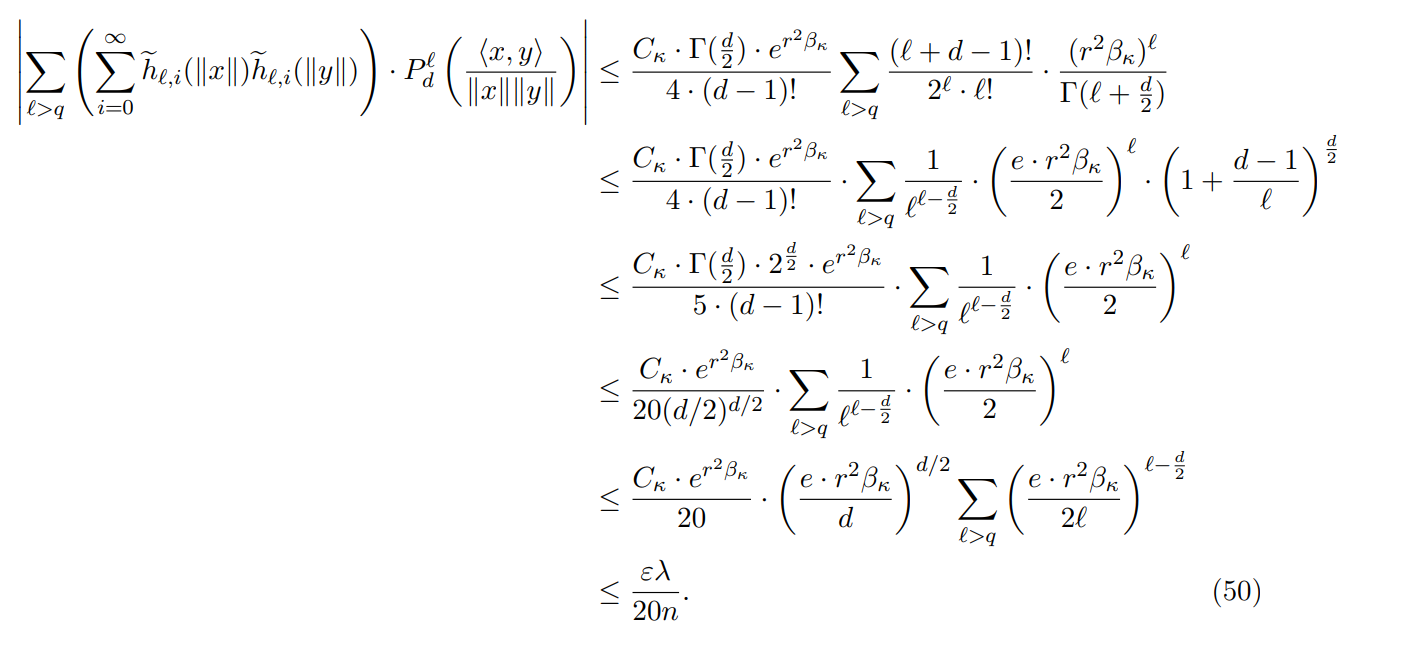
\includegraphics[width=0.99\linewidth]{Figure/설명점해다오.PNG}
    \end{figure}
아마도  $\ell >>d$ 가정 들어간듯, $n! = \Theta(\sqrt{n} (n/e)^n)$
\end{frame}
\begin{frame}{}
\bblue{Gautschi inequality.}
\begin{equation*}
    x^{1-s} < \frac{\Gamma(x+1)}{\Gamma(x+s)} < (x+1)^{1-s}, \quad  x>0, 0<s<1
\end{equation*}
\hrule 
\begin{align*}
    \text{Tail term}&\leq \frac{C_k \cdot e^{r^2 \beta_k}}{20} \cdot \left( \frac{e \cdot r^2 \beta_k}{d} \right)^{d/2} \sum_{\ell > q} \left( \frac{e \cdot r^2 \beta_k}{2 \ell} \right)^{\ell -\frac{d}{2}} \\ 
    &\leq \frac{C_k \cdot e^{r^2 \beta_k}}{20} \cdot \left( \frac{e \cdot r^2 \beta_k}{d} \right)^{d/2} \sum_{\ell > q} \left( \frac{e \cdot r^2 \beta_k}{ \red{2 \ell}} \right)^{\blue{\ell}}   \cdot \left( \frac{1}{\ell} \right)^{-\frac{d}{2}} \cdot \left(\frac{1}{2}\right)^{- \frac{d}{2}}
\end{align*}
\begin{equation*}
\red{\ell} \gets {3.7r^2 \beta_k} \quad \blue{\ell} \gets r^2 \beta_k + \frac{d}{2} \log \frac{3r^2 \beta_k}{d} + \log \frac{C_{\kappa}n}{\varepsilon \lambda}
\end{equation*}
정확히는 \red{$\ell$}을 대입하고 나서 summation 안에 term이 $e^{\blue{-\ell}}$ 이 되니까 실제 $q$보다 작아서 upper-bound를 잡게 됨.  
\end{frame}
\begin{frame}{}
\bgreen{Frullani integral.}
\begin{equation*}
    \int_0^{\infty} \frac{f(ax) - f(bx)}{x} \dd{x} = [f (\infty) - f(0)] \log \frac{a}{b}
\end{equation*}
\end{frame}
\begin{frame}[allowframebreaks]{적분놀이}
\begin{align*}
    \int_0^{\infty} \frac{1- e^{-x}(1+x)}{x(e^x-1)(e^x+e^{-x})} \dd{x} &= \int_0^{\infty} \frac{e^{x} - (1+x)}{x(e^x-1)(e^{2x}+1)} \dd{x} \\ 
    &= \int_0^{\infty} \sum_{k=2}^{\infty} \frac{x^{k-1}}{k!} \sum_{j=1}^{\infty} \left( \frac{1}{k(4j-1)^k} + \frac{1}{k (4j)^k} \right)  \\ 
    &\overset{a}{=} \sum_{j=1}^{\infty} \sum_{k=2}^{\infty} \left( \frac{1}{ k (4j-1)^k} + \frac{1}{k (4j)^k} \right)  \\
    &\overset{b}{=} \sum_{j=1}^{\infty} \left[ \log \left( \frac{4j-1}{4j-2} \right) - \frac{1}{4j-1}\right] + 
    \sum_{j=1}^{\infty} \left[ \log \left(\frac{4j}{4j-1}\right) - \frac{1}{4j}\right]   
\end{align*}
$(a):$ perform the integral using the Gamma integral \\
$(b): \log (1-x) = - \sum_{r=1}^{\infty} \frac{x^r}{r}$ for $-1 \leq x <1$ \\ 
$(c): \prod_{k=1}^{n-1} (k+x) = \frac{\Gamma(n+x)}{\Gamma(1+x)}$, gautschi's inequality
\end{frame}
\section{Stochastic Chebyshev Gradient for Spectral Optimization}
\begin{frame}{}
\bgreen{Lemma.} Then, for any $\vv \in \real^d$, it holds that 
\begin{equation*}
    \nabla_{\theta} \vv^{\top} p_n(\mA) \vv = 2 \sum_{i=0}^{n-1} (2- \mathbf{1}_{i=0}) \vw_i \left( \sum_{j=1}^{n-1} b_{j+1} \vy_{j-i} \right)^{\top} \theta, 
\end{equation*}
where $\vw_{j+1} = 2 \mA \vw_j - \vw_{j-1}, \vw_1 = \mA \vv, \vw_0 = \vv$ and $\vy_{j+1} = 2\vw_{j+1} + \vy_{j-1}, \vy_1 = 2 \mA \vv, \vy_0 = \vv$ \\~\\
$\sum_{j=0}^{\infty} (2- \mathbf{1}_{k=0} \vw_k \vy_{j-k}^{\top}) = \sum_{k=0}^j (2 - \mathbf{1}_{k=0} \vy_{j-k} \vw_k^{\top}) \gets$ \red{이거 진작에 $2w_1=y_1, w_0 =y_0$ 대입하니까 쉽네} 
\end{frame}
\begin{frame}{Trace estimator}
\bgreen{Lemma.}
\begin{equation*}
    \Var_{\vv}[\vv^{\top} \mA \vv] = 2 \left( \norm{\mA}_F^2 - \sum_{i=1}^d \mA_{ii}^2 \right) \leq 2 \norm{\mA}_F^2 
\end{equation*}
for Rademacher random variable $\vv \in [-1,1]^d$ and $\mA \in \cS^{d \times d}$. \\~\\
For Frobenius norm\\ 
\begin{equation*}
\sum_{i=1}^{d^{\prime}} \norm{\frac{\partial \mA}{\partial  \theta_i}}_F^2 = \norm{\frac{\partial \mA}{\partial \theta}}_F^2   
\end{equation*}
right? 
\end{frame}
\begin{frame}{How to deal with infinite-dimensional programming?}
문제: KKT theorem을 infinite-dimensional problem에 적용할 수 없음. 
\begin{enumerate}
    \item 먼저 Finite version의 solution를 구한다. Solution의 limit $q^*$ 를 구한다. 
    \item Objective function이 continuous 한 것을 보이고, feasible set이 non-decreasing set인 것을 보인다. 
    \item Berge의 maximum theorem에 의해서 finite version의 minimum이 infinite version으로 converge한다.  
    \item Step 1에서 구한 $q^*$ 가 minimizer라는 것을 보인다. 
\end{enumerate}
\end{frame}
\begin{frame}{Lemma}
\begin{lemma}
    Suppose that $q_n^*$ is the optimal degree distribution and $b_j$ is the Chebyshev coefficient of the analytic function $f$. Define the weighted coefficient $\hat{b}_j$ as $\hat{b}_j = b_j / (1- \sum_{i=0}^{j-1} q_i^*)$ for $j \geq 0$ (with convention $q_{-1}^* =0 $). Then, there exists constants $D_1^{\prime}, D_2^{\prime} > 0 $ independent of $M,N$ such that 
    \begin{equation*}
        \sum_{n=1}^{\infty} q_n \left( \sum_{j=1}^{\infty} |\hat{b}_j| j^4| \right)^2 \leq D_1^{\prime} + \frac{D_2^{\prime} N^8}{\rho^{2N}}
    \end{equation*}
\end{lemma}
\bgreen{어디다 써먹음?} \\ 
\begin{equation*}
    \E_{n, \vv} [ \norm{\psi - \psi^{\prime}}_2^2 ] \leq D_0 \left( \frac{L_A^4 + \beta_A^2}{M} + L_A^4 \right) \norm{\Delta \theta}_2^2 \E_n \left[ \left( \sum_{j=1}^{n} |\abs{\hat{b}_j^2} j^4 \right) \right]
\end{equation*} 
비슷한 Lemma는 여기다 적용 $N \gets \sqrt{N}$
\begin{equation*}
    \E_{n,v} [\psi^2] \leq \frac{4}{(b-a)^2} \left( \frac{2 L_A^2}{M} + d^{\prime} L_{nuc}^2 \right) \E_n \left[ \left( \sum_{j=1}^n \abs{\hat{b}_j} j^2 \right)^2 \right]
\end{equation*}
\end{frame}
\begin{frame}{About Chebyshev Polynomial}
\begin{lemma}
    Suppose that $A, A+E \in \real^{d \by d}$ are symmetric matrices and they have eigenvalues in $[-1,1]$. Let $T_i$ and $U_i$ be the first and the second kind of Chebyshev basis polynomial with degree $i \geq 0$, respectively. Then, is holds that 
    \begin{equation*}
        \norm{T_i (A+E) - T_i (A)} \leq i^2 \norm{E}, \quad \norm{U_i (A+E) - U_i (A)} \leq \frac{i (i+1) (i+2) }{3} \norm{E}
    \end{equation*}
    where $\norm{\cdot}$ can be $\norm{\cdot}_2$ (spectral norm) or $\norm{\cdot}_2$ (Frobenius norm) 
\end{lemma}
$T_i$ 는 $i^2$-Lipschitz 이고 $U_i$ 는 $\frac{i (i+1)(i+2)}{3}$-Lipschitz 이다. 
\end{frame}
\begin{frame}{Lemma}
\begin{figure}
    \centering
    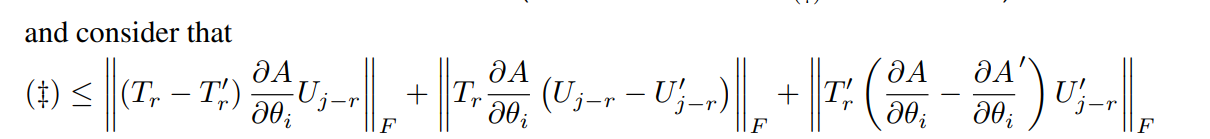
\includegraphics[width=0.9\linewidth]{Figure/typo.PNG}
\end{figure}
\red{아무리 봐도 두 번째 term $T_r$ 대신 $T_r^{\prime}$ 이 와야한다}
\begin{figure}
    \centering
    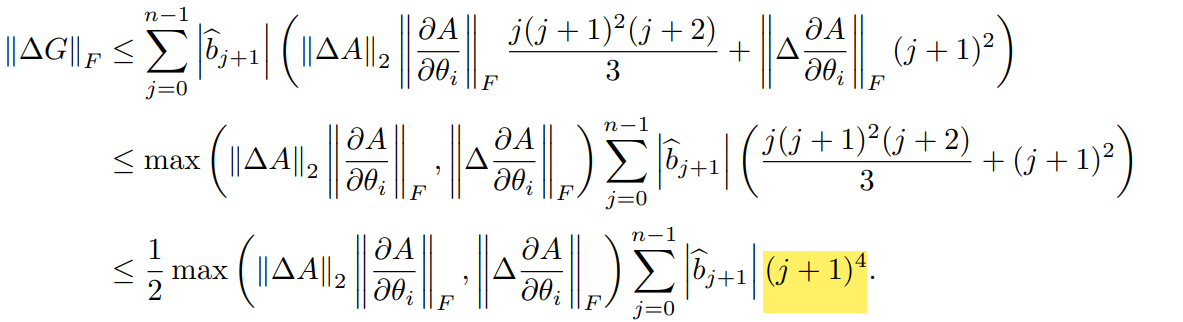
\includegraphics[width=.9\linewidth]{Figure/ty2.PNG}
\end{figure}
\blue{계산 적당히 하고 $(j+1)^4$로 묶어라}
\end{frame}

\end{document}